\documentclass{article}
% Útgáfa 1.5

% pakkar fyrir töflur; array er notað í "math-mode"; arydshln fyrir brotalínur í töflum
\usepackage{array,tabularx}%,arydshln}  
% íslenskt letur, orðaskiptingar ...
\usepackage[english]{babel}
\usepackage[T1]{fontenc}
% númera jöfnur, töflur, myndir, ...
\usepackage{enumerate}
% fyrir krækjur
\usepackage[colorlinks,linkcolor=blue,citecolor=blue,urlcolor=blue]{hyperref}
% ýmis tákn, leturgerðir, ... ATH amsmath fyrir \text{} skipunina
\usepackage{amsmath,amssymb,euscript}   
% til að setja inn *.eps myndir ef við notum dvi og ps skjöl...
\usepackage{epsfig}    % \epsfig{...}
% ... en ef við notum pdf beint, þá er þetta pakkinn sem við þurfum
\usepackage{graphicx}  % \includegraphics[...]{...}
% litamöguleikar fyrir texta
\usepackage{color}
% til þess að myndir og töflur standi þar sem þær eiga að standa!
\usepackage{here}
%
\setlength{\textwidth}{7in}
\setlength{\textheight}{9in}
\setlength{\headheight}{0in}
\setlength{\headsep}{6pt}
\setlength{\topskip}{0in}
\setlength{\topmargin}{0cm}
\setlength{\oddsidemargin}{-0.3in}
\setlength{\marginparwidth}{10pt}
% dregur fyrstu línu í hverri málsgrein inn - nota 0cm fyrir engan inndrátt fyrir allar málsgreinar en \noindent í upphafi málsgreinar til að hafa engan inndrátt í þeirri málsgrein einni:
\setlength{\parindent}{0cm}
% viljum hafa eitt línubil milli efnisgreina
\setlength{\parskip}{1.5ex plus 0.75ex minus 0.5ex}
% 1.5 í línubil
\renewcommand{\baselinestretch}{1.025}

% Environments
\newenvironment{alist}[1][$\quad\,$1.]{
\vspace*{-8pt} \begin{enumerate}[label=\alph*),itemsep=4pt,parsep=3pt]}
{\end{enumerate}\vspace*{-3pt}}

\newenvironment{ttafla}[1][$\quad\,$1.]{
\begin{tabular}{rcl} \renewcommand\arraystretch{2} }
{\end{tabular}}



%Bætt við af mér (Hannesi)
% Þjappa saman
\widowpenalty=600
\clubpenalty=600
\usepackage[compact]{titlesec}
\titlespacing{\section}{0pt}{2ex plus 0.75ex minus 0.75ex}{1ex plus 0.3ex minus 0.3ex}
\titlespacing{\subsection}{0pt}{1ex plus 0.25ex minus 0.25ex}{0ex plus 0.1ex minus 0.1ex}
\titlespacing{\subsubsection}{0pt}{0.5ex plus 0.1ex minus 0.1ex}{0ex plus 0.1ex minus 0.1ex}

% Bolda caption
\usepackage[hang,small,bf]{caption}

% Efnaformúlur og myndir
%\usepackage[version=3]{mhchem}
\usepackage{chemfig}

% Komma í stað punkts
\usepackage{icomma}

% Annað
\usepackage{subfig}
\usepackage{array}
\usepackage{bigstrut}
\usepackage{multirow}
\usepackage{multicol}
\usepackage{enumerate}
%\usepackage{enumitem}
\usepackage{wrapfig}
\newcommand{\HRule}{\rule{\linewidth}{0.5mm}}
\usepackage{ulem}
%\usepackage[thinspace,mediumqspace,amssymb]{SIunits}

%Tikz
\usepackage{tikz}
\usetikzlibrary{fit,arrows,decorations.pathmorphing,decorations.text,backgrounds,positioning,fit,petri,3d,calc}
%% 3d hnitakerfi
\usepackage{tikz-3dplot}
\tdplotsetmaincoords{75}{130}
%\begin{tikzpicture}[scale=5,tdplot_main_coords]
%
%%set up some coordinates 
%%-----------------------
%\coordinate (O) at (0,0,0);
%
%%determine a coordinate (P) using (r,\theta,\phi) coordinates.  This command
%%also determines (Pxy), (Pxz), and (Pyz): the xy-, xz-, and yz-projections
%%of the point (P).
%%syntax: \tdplotsetcoord{Coordinate name without parentheses}{r}{\theta}{\phi}
%\tdplotsetcoord{P}{\rvec}{\thetavec}{\phivec}


%%%%%%%%%%%%%%% SKIPANIR %%%%%%%%%%%%%%%%%%%%%%%%
%% LITASTYTTINGAR
%
\definecolor{dgreen}{rgb}{0,0.8,0}
\newcommand{\red}[1]{{\color{red} #1}}
\newcommand{\green}[1]{{\color{dgreen} #1}}
\newcommand{\blue}[1]{{\color{blue} #1}}
\newcommand{\black}[1]{{\color{black} #1}}
%
% ALLS KYNS STÆRÐFRÆÐIDÓT
%
\newcommand{\lvec}{\overrightarrow}
%
% ýmsar diffurstyttingar
\newcommand{\dif}{\,\mathrm{d}}
\newcommand{\dx}{\,\mathrm{d}x}
\newcommand{\dy}{\,\mathrm{d}y}
\newcommand{\dz}{\,\mathrm{d}z}
\newcommand{\dt}{\,\mathrm{d}t}
% afleiður og hlutafleiður
\renewcommand{\d}[2]{\frac{\dif{#1}}{\dif{#2}}}
\newcommand{\dd}[3]{\frac{\dif^{#1}{#2}}{\dif^{#1}{#3}}}
\newcommand{\p}[2]{\frac{\partial{#1}}{\partial {#2}}}
\newcommand{\pp}[3]{\frac{\partial^{#1}{#2}}{\partial{#3}^{#1}}}
%
% bil, millistig \; og \quad
\newcommand{\bil}{\hspace*{6pt}}
\newcommand{\Bil}{\hspace*{10pt}}
\newcommand{\vbil}{\vspace*{-6pt}}
\newcommand{\vBil}{\vspace*{-10pt}}

% samasemmerki með aukaplássi á báða bóga
\newcommand{\bils}{\bil=\bil}
%
\newcommand{\bc}{\begin{center}}
\newcommand{\ec}{\end{center}}
%
\newcommand{\beq}{\begin{equation}}
\newcommand{\eeq}{\end{equation}}
%
\newcommand{\beqa}{\begin{eqnarray*}}
\newcommand{\eeqa}{\end{eqnarray*}}
%
\newcommand{\ba}{\begin{array}}
\newcommand{\ea}{\end{array}}
%
\newcommand{\bma}{\begin{matrix}}
\newcommand{\ema}{\end{matrix}}
%
\newcommand{\bmh}{\left[\begin{matrix}}
\newcommand{\emh}{\end{matrix}\right]}
%
\newcommand{\ts}{\textstyle}
\newcommand{\ds}{\displaystyle}

% Frá mér (Hannesi)
\newcommand{\lausn}{\textbf{\textit{Lausn:}}}
\newcommand{\solution}{\textbf{\textit{Solution:}}}
\newcommand{\daemi}{\textbf{\textit{Dæmi:}}}
\newcommand{\bt}{\begin{table}[H]}
\newcommand{\et}{\end{table}}
\newcommand{\atm}{\text{atm}}
\newcommand{\calories}{\text{cal}}
\everymath{\displaystyle} % Svo allar jöfnur taka aldrei minna pláss
\renewcommand\tabcolsep{2pt} % Bil dalka í töflum
\setlength{\arraycolsep}{1.5pt}
%\usepackage{fancyhdr}
%\setlength{\headheight}{25pt}
%\pagestyle{fancy}
%\renewcommand{\headrulewidth}{0.4pt}
%\renewcommand{\footrulewidth}{0.4pt}
%\usepackage[top=2.5in, bottom=1.5in, left=1in, right=1in]{geometry}
\usepackage{amssymb}
\usepackage{pifont}
\newcommand{\cmark}{\text{\ding{51}}}%
\newcommand{\xmark}{\text{\ding{55}}}%

\usepackage{pbox}
%\usepackage{fancyvrb}
\usepackage{array}
\newcolumntype{L}[1]{>{\raggedright\let\newline\\\arraybackslash\hspace{0pt}}m{#1}}
\newcolumntype{C}[1]{>{\centering\let\newline\\\arraybackslash\hspace{0pt}}m{#1}}
\newcolumntype{R}[1]{>{\raggedleft\let\newline\\\arraybackslash\hspace{0pt}}m{#1}}
\usepackage[utf8]{inputenc}
\usepackage{framed}
\usepackage{paralist}
\renewenvironment{enumerate}[1]{\begin{compactenum}#1}{\end{compactenum}}
\usetikzlibrary{shapes.multipart,positioning,arrows}

\begin{document}
\begin{titlepage}
\begin{center}
\textsc{}\\[2cm] 

\includegraphics[width=6cm]{Haskoli_Islands_rett.jpg}\\[0.5cm]
\HRule \\[0.6cm]
{ \huge \bfseries Group assignment 4: Refined OO model}\\[0.2cm]
\HRule \\[0.4cm]
\textsc{\normalsize Þróun hugbúnaðar} \\
\textsc{Spring 2015} \\[1.5cm]
\begin{minipage}{0.45\textwidth}
\begin{flushleft} \large
\textit{Students:} (Group F2a)\\
\textsc{Einar Helgi Þrastarson} \\
\textsc{Hannes Pétur Eggertsson} \\
\textsc{Sigurður Birkir Sigurðsson} \\
\end{flushleft}
\end{minipage}
\begin{minipage}{0.45\textwidth}
\begin{flushright} \large
\textit{Teachers:} \\
\textsc{Matthias Book}\\
\textsc{Kristín Fjóla Tómasdóttir}\\
\textsc{ }\\
\end{flushright}
\end{minipage}

\end{center}
\end{titlepage}


% Description of the project
\section{Introduction}
In this document there's the class diagram for group F2a. Group members are: Einar Helgi Þrastarson (personal ID number: 110287-2919), Hannes Pétur Eggertsson (240889-2939) and Sigurður Birkir Sigurðsson (120589-2539). Our project is to build an user interface for a fantasy football game. In our class diagram we felt it made sense to split the classes into two categories, back-end classes and front-end classes. Then, in a third diagram there's another diagram that shows the connections between the back-end and  We will all present this document on Wednesday, March ?th 2015.

\subsection{Notation}
In our class diagrams we use the following notation:\vspace*{-0.3cm}
\begin{itemize}\itemsep-4pt
\item[--] means a private variable or method (not directly accessable by other classed).
\item[+] means a public variable or method (directly accessable by other classes).
\end{itemize}

\tikzset{umlclass/.style={
        draw=black,fill=yellow!16,rectangle split,align=center, rectangle split part align={center,left}, minimum width=4cm,rounded corners},draw,rectangle split parts=4}

Each class in the diagram has four sections shown below:
\begin{center} \vspace*{-0.15cm}
\begin{tikzpicture}
\begin{scope}[xshift=8cm,yshift=0cm]
\node[umlclass] (t1)
 {\textbf{\large \textit{The class' name.}}
 \nodepart{two}
  {\footnotesize
  \begin{tabular}{l} 
   Short description of the class.
  \end{tabular}}
 \nodepart{three}
  \begin{tabular}{l}
  The class' variables and their type listed\\
  on the format:\\
   --/+ \texttt{type1 variable1}\\
   --/+ \texttt{anotherClass variable2}\\
  \end{tabular}
 \nodepart{four}
  \begin{tabular}{l}
   The class' methods listed on the format:\\
   --/+ \texttt{type1 method1(type variable,...)}\\
   --/+ \texttt{type2 method2(...)}\\
  \end{tabular}
 };
\end{scope}
\end{tikzpicture}
\end{center}\vspace*{-0.15cm}
If the class wasn't created by us it is filled with red. Back-end classes are green and front-end classes are yellow. Classes are interconnected using arrows:

\begin{tikzpicture}
\draw[arrows={-angle 60},thick] node[left]{Class A} (0,0) to (3,0)node[draw=none,midway,above=0cm] {\hspace*{3cm}\textit{uses}} node[right]{Class B};
%\begin{scope}[yshift=-0.8cm]
%\draw[arrows={-open triangle 60},thick] node[left]{Class A} (0,0) to (3,0)node[draw=none,midway,above=0cm] {\hspace*{3cm}\textit{extends}} node[right]{Class B};
%\end{scope}
%\begin{scope}[yshift=-1.6cm]
%\draw[arrows={-triangle 60},thick] node[left]{Class A} (0,0) to (3,0)node[draw=none,midway,above=0cm] {\hspace*{3cm}\textit{implements}} node[right]{Class B};
%\end{scope}
\end{tikzpicture}

In most cases we can tell how many classes 'Class A' and 'Class B' will be associated with, this is shown by placing an arrow at the beginning and end of an arrow, e.g.

\begin{tikzpicture}
\draw[arrows={-angle 60},thick] node[left]{Class A} node[above right]{1} (0,0) to (3,0)node[draw=none,midway,above=0cm] {\hspace*{3cm}\textit{uses}} node[above left]{0--10} node[right]{Class B};
\end{tikzpicture}

if each instance of 'Class A' will use 'Class B' in a range of 0 to 10 instances. If no numbers are shown it generally means the association is 1 uses 1.

\section{Class diagram}
We decided to split our class diagram into two figures: \textbf{Back-end classes} and \textbf{Front-end classes}. The back-end classes take care of storing and keeping track of all information as the game is running. The front-end classes take care of displaying the information to the users playing the game as well as handling their input.

\subsection{Back-end classes}
\begin{tikzpicture}
%% ==========================================
%% User
%% ==========================================
\begin{scope}[yshift=1cm]
\node[umlclass,fill=green!26] (user)
 {\textbf{\large \textit{User}}
 \nodepart{two}
  {\footnotesize
  \begin{tabular}{l} 
   This class keeps track of all information about\\
   each user playing the game.\\
   
  \end{tabular}}
 \nodepart{three}
  \begin{tabular}{l}
   -- \texttt{int id}\\
   -- \texttt{int money}\\
   -- \texttt{int score}\\
   -- \texttt{int roundscore}\\
   -- \texttt{String name}\\
   -- \texttt{Roster roster}\\
  \end{tabular}
 \nodepart{four}
  \begin{tabular}{l}
   + \texttt{User(String name, int id)}\\
   + \texttt{int getMoney()}\\
   + \texttt{boolean isAffordable(int price)}\\
   + \texttt{void changeMoney(int dMoney)}\\
   + \texttt{Roster getRoster()}\\
   + \texttt{int getScore()}\\
   + \texttt{int getRoundScore()}\\
   + \texttt{void setScore(int newscore)}\\
   + \texttt{String getName()}\\
   + \texttt{void setName(String newname)}\\ 
  \end{tabular}
 };
\end{scope}

%% ==========================================
%% Roster
%% ==========================================
\begin{scope}[xshift=10cm,yshift=0.1cm]
\node[umlclass,fill=green!26] (roster)
 {\textbf{\large \textit{Roster}}
 \nodepart{two}
  {\footnotesize
  \begin{tabular}{l} 
   Keeps track of which football players are in which user team/roster.
  \end{tabular}}
 \nodepart{three}
  \begin{tabular}{l}
   -- \texttt{List<Player> goalkeepers}\\
   -- \texttt{List<Player> goalkeepersOnField}\\
   -- \texttt{List<Player> defenders}\\
   -- \texttt{List<Player> defendersOnField}\\
   -- \texttt{List<Player> midfielders}\\
   -- \texttt{List<Player> midfieldersOnField}\\
   -- \texttt{List<Player> forwards}\\
   -- \texttt{List<Player> forwardsOnField}\\
   -- \texttt{int numberOfPlayersOnField}\\
  \end{tabular}
 \nodepart{four}
  \begin{tabular}{l}
   + \texttt{Roster()}\\
   + \texttt{int getNumberOfPlayersOnField()}\\
   + \texttt{boolean removePlayerFromField(Player player)}\\
   + \texttt{void removePlayerFromRoster(Player player)}\\
   -- \texttt{void removePlayer(Player p, boolean fromRoster)}\\
   + \texttt{boolean addPlayerToField(Player player)}\\
   + \texttt{boolean addPlayerToRoster(Player player)}\\
   + \texttt{List< List<Player> > getPlayersInRoster()}\\
   + \texttt{List< List<Player> > getPlayersOnField()}\\
   + \texttt{boolean isInRoster(Player player)}\\
   + \texttt{boolean isOnField(Player player)}\\
  \end{tabular}
 };
\end{scope}

%% ==========================================
%% MainGame
%% ==========================================
\begin{scope}[yshift=-7.68cm]
\node[umlclass,fill=green!26] (maingame)
 {\textbf{\large \textit{MainGame}}
 \nodepart{two}
  {\footnotesize
  \begin{tabular}{l} 
   The main back-end class. Keeps track of\\
   the state of the game. It exists always\\
   while the game is running.
  \end{tabular}}
 \nodepart{three}
  \begin{tabular}{l}
   -- \texttt{static final MainGame game}\\
   -- \texttt{StatsHistory stats}\\
   -- \texttt{List<User> users}\\
   -- \texttt{int round}\\
   -- \texttt{int currentUser}\\
  \end{tabular}
 \nodepart{four}
  \begin{tabular}{l}
   -- \texttt{static MainGame()}\\
   + \texttt{MainGame getInstance()}\\
   + \texttt{void setNumUsers(int num)}\\
   + \texttt{void nextUser()}\\
   + \texttt{int getRound()}\\
   + \texttt{List<User> getUsers()}\\
   + \texttt{StatsHistory getStatsHistory()}\\
   + \texttt{User getCurrentUser()}\\
  \end{tabular}
 };
\end{scope}

%% ==========================================
%% Player
%% ==========================================
\begin{scope}[xshift=8.5cm,yshift=-7.4cm]
\node[umlclass,rectangle split parts=3,fill=red!32] (player)
 {\textbf{\large \textit{Player} <<interface>>}
 \nodepart{two}
  {\footnotesize
  \begin{tabular}{l} 
   This class will be made by group F1a. Each\\
   instance will contain information about a\\
   football player. It will (at least)git pull have the\\
   following instance variables and functions.
  \end{tabular}}
 \nodepart{three}
  \begin{tabular}{l}
   -- \texttt{enum Position}\\
   + \texttt{String getName()}\\
   + \texttt{Integer getPrice()}\\
   + \texttt{Position getPosition}
  \end{tabular}
 \nodepart{four}
 };
\end{scope}

%% ==========================================
%% StatsHistory
%% ==========================================
\begin{scope}[xshift=10cm,yshift=-13cm]
\node[umlclass,fill=green!26] (statshistory)
 {\textbf{\large \textit{StatsHistory}}
 \nodepart{two}
  {\footnotesize
  \begin{tabular}{l} 
   A class that hold on to statistical information for objects with scores.
  \end{tabular}}
 \nodepart{three}
  \begin{tabular}{l}
   -- \texttt{List<ObjectScores> allplayerscores}\\
   -- \texttt{List<ObjectScores> alluserscores}\\
  \end{tabular}
 \nodepart{four}
  \begin{tabular}{l}
  + \texttt{StatsHistory()}\\
  + \texttt{void createPlayerScoreObject(Object player)}\\
  + \texttt{void createUserScoreObject(Object user)}\\
  + \texttt{List<Integer> getPlayerScores(Player player)}\\
  + \texttt{List<Integer> getUserScores(User user)}\\
  - \texttt{List<Integer> getUserScores(User user, boolean total)}\\
  + \texttt{void addScoreToPlayer(Player player, int score)}\\
  + \texttt{void addScoreToUser(User user, int score)}\\
  \end{tabular}
 };
\end{scope}

%% ==========================================
%% ObjectScores
%% ==========================================
\begin{scope}[xshift=0cm,yshift=-14.5cm]
\node[umlclass,fill=green!26] (playerscores)
 {\textbf{\large \textit{ObjectScores}}
 \nodepart{two}
  {\footnotesize
  \begin{tabular}{l} 
   A class to add scores to an object.
  \end{tabular}}
 \nodepart{three}
  \begin{tabular}{l}
   -- \texttt{Object object}\\
   -- \texttt{List<Integer> scores}\\
   -- \texttt{List<Integer> totalscores}
  \end{tabular}
 \nodepart{four}
  \begin{tabular}{l}
   + \texttt{ObjectScores(Object object)}\\
   + \texttt{void addScore(int score)}\\
   + \texttt{List<Integer> getScores()}\\
   + \texttt{List<Integer> getTotalScores()}\\
   + \texttt{Object getObject()}
  \end{tabular}
 };
\end{scope}

%% ==========================================
%% Allar örvar teiknaðar hér
%% ==========================================
% user to roster
\draw[arrows={-angle 60},thick] ([yshift=-20pt]user.three east) node[right]{1} to [out=45, in=-150](roster.text west) node[above left]{1};

% maingame to user
\draw[arrows={-angle 60},thick]
[out=0, in=90](maingame.three east) node[right=0.15cm]{1} to [out=75, in=-75](user.text east) node[right]{1--N};

% maingame to statshistory
\draw[arrows={-angle 60},thick]
[out=0, in=90]([yshift=0.5cm]maingame.three east) node[right=0.15cm]{1} to [out=-65, in=111](statshistory.text west) node[left]{1};

% roster to player
\draw[arrows={angle 60-},thick] (player.text west) to [out=105, in=-120]([yshift=-1cm]roster.three west);

% StatsHistory to PlayerScores
\draw[arrows={-angle 60},thick] ([yshift=0.2cm]statshistory.three west) node[above left]{1} to [out=-135, in=10](playerscores.text east) node[below right]{$P$};

% StatsHistory to Player (backwards)
\draw[arrows={angle 60-},thick] ([yshift=0.2cm]statshistory.four west) to [out=110, in=-120](player.text west);
\end{tikzpicture}  
$N$ is er number of total users in the current game and $P$ is the total amount of football players in the game.

\newpage
\subsection{Front-end classes}
\begin{tikzpicture}
%% ==========================================
%% Start Panel
%% ==========================================
\begin{scope}[xshift=11.5cm,yshift=1.52cm]
\node[umlclass] (startpanel)
 {\textbf{\large \textit{StartPanel}}
 \nodepart{two}
  {\footnotesize
  \begin{tabular}{l} 
   StartPanel will be spawned at the very start \\
   of the game. It will ask users to type in their\\
   name before the game begins.
  \end{tabular}}
 \nodepart{three}
  \begin{tabular}{l}
   -- \texttt{JPanel center}\\
   -- \texttt{JTextField field}\\
   -- \texttt{List<String> names}\\
   -- \texttt{int numEmpty}\\
   -- \texttt{JButton startGame}\\
   -- \texttt{JButton addPlayer}\\   
  \end{tabular}
 \nodepart{four}
  \begin{tabular}{l}
   + \texttt{StartPanel()}\\
   + \texttt{addPlayerHandler()}\\
   + \texttt{void changeCenter()}\\
  \end{tabular}
 };
\end{scope}

%% ==========================================
%% LeaguePanel
%% ==========================================
\begin{scope}[xshift=11cm,yshift=-15.7cm]
\node[umlclass,rectangle split parts=3] (leaguepanel)
 {\textbf{\large \textit{LeaguePanel}}
 \nodepart{two}
  {\footnotesize
  \begin{tabular}{l} 
   The panel that shows the users the current league \\
   standings, and which games are upcoming.
  \end{tabular}}
 \nodepart{three}
  \begin{tabular}{l}
   + \texttt{LeaguePanel()}\\
  \end{tabular}
 };
\end{scope}

%% ==========================================
%% FieldViewer Panel
%% ==========================================
\begin{scope}[xshift=10.3cm,yshift=-12.4cm]
\node[umlclass] (fieldviewerpanel)
 {\textbf{\large \textit{FieldViewerPanel}}
 \nodepart{two}
  {\footnotesize
  \begin{tabular}{l} 
   This class shows the current user his roster\\
   on a football field.
  \end{tabular}}
 \nodepart{three}
  \begin{tabular}{l}
   -- \texttt{final JPanel[] players}\\
   -- \texttt{final Roster roster}\\
  \end{tabular}
 \nodepart{four}
  \begin{tabular}{l}
   + \texttt{FieldViewerPanel()}\\
   + \texttt{JLabel createLabels(String name)}\\
   + \texttt{void paintComponent(Graphics g)}\\
  \end{tabular}
 };
\end{scope}

%% ==========================================
%% Market Panel
%% ==========================================
\begin{scope}[xshift=10.5cm,yshift=-5.9cm]
\node[umlclass] (marketpanel)
 {\textbf{\large \textit{MarketPanel}}
 \nodepart{two}
  {\footnotesize
  \begin{tabular}{l} 
   Shows the user the market of players which he/she can buy\\
   or sell.
  \end{tabular}}
 \nodepart{three}
  \begin{tabular}{l}
   -- \texttt{final JTextField field}\\
   -- \texttt{String player\_choice}\\
   -- \texttt{String team\_choice}\\ 
   -- \texttt{String pos\_choice}\\
   -- \texttt{JTable jtable}\\
   -- \texttt{JScrollPane scroll}\\ 
   -- \texttt{JPanel wrapper}\\
   -- \texttt{List<Player> results}\\ 
  \end{tabular}
 \nodepart{four}
  \begin{tabular}{l}
   + \texttt{MarketPanel(JScrollPane scroll, int val)}\\
   + \texttt{JComboBox<String> addComboBox(}\\
   \texttt{\hspace*{0.4cm}List<String> choices, String flag)}\\
   -- \texttt{void refreshJTable()}\\
   -- \texttt{JTable getJTable(String player\_searchd,}\\
   \texttt{\hspace*{0.4cm}String team\_searchd, String pos\_searchd)}\\
   -- \texttt{Object[][] getTableData()}\\
  \end{tabular}
 };
\end{scope}

%% ==========================================
%% Roster Panel
%% ==========================================
\begin{scope}[xshift=0cm,yshift=-14.9cm]
\node[umlclass] (rosterpanel)
 {\textbf{\large \textit{RosterPanel}}
 \nodepart{two}
  {\footnotesize
  \begin{tabular}{l} 
   Shows the players his current roster and the status\\
   of his/her players, e.g. injuries and yellow/red cards.
  \end{tabular}}
 \nodepart{three}
  \begin{tabular}{l}
   -- \texttt{Roster roster}\\
   -- \texttt{JLabel num\_players}\\
   -- \texttt{final Integer IS\_ON\_FIELD\_COLUMN}\\ 
  \end{tabular}
 \nodepart{four}
  \begin{tabular}{l}
   + \texttt{RosterPanel()}\\
  \end{tabular}
 };
\end{scope}

%% ==========================================
%% Score Panel
%% ==========================================
\begin{scope}[xshift=6.3cm,yshift=-0.6cm]
\node[umlclass,rectangle split parts=3] (scorepanel)
 {\textbf{\large \textit{ScorePanel}}
 \nodepart{two}
  {\footnotesize
  \begin{tabular}{l} 
   Shows all user's scores and\\
   shows GraphDataPanel.
  \end{tabular}}
 \nodepart{three}
  \begin{tabular}{l}
   + \texttt{ScorePanel()}\\
  \end{tabular}
 };
\end{scope}

%% ==========================================
%% NameChange Panel
%% ==========================================
\begin{scope}[xshift=-0.3cm,yshift=-10.7cm]
\node[umlclass] (namechange)
 {\textbf{\large \textit{NameChangePanel}}
 \nodepart{two}
  {\footnotesize
  \begin{tabular}{l} 
   Allows the user to change his/her name,\\
   also shows some key information: current\\
   player, money, and round. 
  \end{tabular}}
 \nodepart{three}
  \begin{tabular}{l}
   -- \texttt{final JTextField name}\\
  \end{tabular}
 \nodepart{four}
  \begin{tabular}{l}
   + \texttt{NameChange()}\\
   + \texttt{void changeName(String newName)}\\
   + \texttt{void addChangeListener()}\\
  \end{tabular}
 };
\end{scope}

%% ==========================================
%% GraphData Panel
%% ==========================================
\begin{scope}[xshift=-0.3cm,yshift=-6.6cm]
\node[umlclass] (graphdatapanel)
 {\textbf{\large \textit{GraphDataPanel}}
 \nodepart{two}
  {\footnotesize
  \begin{tabular}{l} 
   Creates a linear graph with the user's score\\
    showing their score after each round.
  \end{tabular}}
 \nodepart{three}
  \begin{tabular}{l}
   -- \texttt{final Color[] col}\\
  \end{tabular}
 \nodepart{four}
  \begin{tabular}{l}
   + \texttt{GraphData()}\\
   + \texttt{void paintComponent(Graphics g)}\\
  \end{tabular}
 };
\end{scope}

%% ==========================================
%% Endgame Panel
%% ==========================================
\begin{scope}[xshift=6.2cm,yshift=3.35cm]
\node[umlclass,rectangle split parts=3] (endgamepanel)
 {\textbf{\large \textit{EndgamePanel}}
 \nodepart{two}
  {\footnotesize
  \begin{tabular}{l} 
   Pops up after the 10th round.\\ 
   Shows the winner and statist-\\
   ics about the game.
  \end{tabular}}
 \nodepart{three}
  \begin{tabular}{l}
   + \texttt{EndgamePanel()}\\
  \end{tabular}
 };
\end{scope}

%% ==========================================
%% Main
%% ==========================================
\begin{scope}[xshift=-0.6cm,yshift=0cm]
\node[umlclass] (main)
 {\textbf{\large \textit{Main}}
 \nodepart{two}
  {\footnotesize
  \begin{tabular}{l} 
   The main front-end class. It is initialized\\
   at the start of the game and runs until the\\
   game is terminated.
  \end{tabular}}
 \nodepart{three}
  \begin{tabular}{l}
   -- \texttt{static final Main instance}\\
   -- \texttt{JFrame frame}\\
   -- \texttt{JPanel right}\\
   -- \texttt{JPanel change}\\
   -- \texttt{MainGame game}\\
  \end{tabular}
 \nodepart{four}
  \begin{tabular}{l}
   -- \texttt{static Main()}\\
   + \texttt{static Main getInstance()}\\
   + \texttt{void setEndgamePanel()}\\
   + \texttt{void startGame()}\\
   + \texttt{void restartFrame()}\\
   + \texttt{void setPanelAsScore()}\\
   + \texttt{void setPanelAsMarket()}\\
   + \texttt{void setPanelAsFieldViewer()}\\
   + \texttt{void setPanelAsLeague()}\\ 
   + \texttt{void setPanelAsRoster()}\\
   + \texttt{Dimension returnPanelSize()}\\
   + \texttt{void main(String[] args)}\\
  \end{tabular}
 };
\end{scope}

%% ==========================================
%% Allar örvar teiknaðar hér
%% ==========================================
% main to startpanel
\draw[arrows={-angle 60},thick] ([yshift=29pt]main.four east) to [out=75, in=-170](startpanel.three west);

% main to endgamepanel
\draw[arrows={-angle 60},thick] ([yshift=40pt]main.four east) to [out=85, in=-110](endgamepanel.text west);

% main to scorepanel
\draw[arrows={-angle 60},thick] ([yshift=5pt]main.four east) to [out=50, in=-150](scorepanel.text west);

% main to marketpanel
\draw[arrows={-angle 60},thick] ([yshift=-6pt]main.four east) to [out=0, in=180](marketpanel.text west);

% main to fieldviewerpanel
\draw[arrows={-angle 60},thick] ([yshift=-17pt]main.four east) to [out=0, in=150](fieldviewerpanel.text west);

% main to leaguepanel
\draw[arrows={-angle 60},thick] ([yshift=-28pt]main.four east) to [out=-10, in=180](leaguepanel.text west);

% main to rosterpanel
\draw[arrows={-angle 60},thick] ([yshift=-39pt]main.four east) to [out=-15, in=80](rosterpanel.text east);

% main to namechangepanel
\draw[arrows={-angle 60},thick] ([yshift=-61pt]main.four east) to [out=-25, in=66](namechange.text east);

% scorepanel to graphdatapanel
\draw[arrows={-angle 60},thick] ([yshift=-26pt]scorepanel.four west) to [out=-165, in=45](graphdatapanel.text east);
\end{tikzpicture}

Multiplicities are all 1:1.

\subsubsection{Component classes}
We are also using the following two component classes

\begin{tikzpicture}
%% ==========================================
%% HandleButtons
%% ==========================================
\begin{scope}[xshift=0cm,yshift=0cm]
\node[umlclass] (HandleButtons)
 {\textbf{\large \textit{HandleButtons}}
 \nodepart{two}
  {\footnotesize
  \begin{tabular}{l} 
   Desc.
  \end{tabular}}
 \nodepart{three}
  \begin{tabular}{l}
  \end{tabular}
 \nodepart{four}
  \begin{tabular}{l}
   + \texttt{void actionPerformed(ActionEvent e)}\\
  \end{tabular}
 };
\end{scope}

%% ==========================================
%% ButtonColumn
%% ==========================================
\begin{scope}[xshift=0cm,yshift=0cm]
\node[umlclass] (ButtonColumn)
 {\textbf{\large \textit{ButtonColumn}}
 \nodepart{two}
  {\footnotesize
  \begin{tabular}{l} 
   Changes a single column of a JTable to buttons.
  \end{tabular}}
 \nodepart{three}
  \begin{tabular}{l}
   -- \texttt{JTable table}\\
   -- \texttt{Action action}\\
   -- \texttt{int mnemonic}\\ 
   -- \texttt{Border originalBorder}\\
   -- \texttt{Border focusBorder}\\
   -- \texttt{JButton renderButton}\\
   -- \texttt{JButton editButton}\\ 
   -- \texttt{Object editorValue}\\
   -- \texttt{boolean isButtonColumnEditor}\\
  \end{tabular}
 \nodepart{four}
  \begin{tabular}{l}
   + \texttt{ButtonColumn(JTable table, Action action, int column)}\\
   + \texttt{Border getFocusBorder()}\\
   + \texttt{void setFocusBorder(Border focusBorder)}\\
   + \texttt{int getMnemonic}\\
   + \texttt{void setMnemonic(int mnemonic)}\\
   + \texttt{Component getTableCellEditorComponent(JTable t, Object val,}\\
    \texttt{\hspace*{0.4cm} boolean selected, int row, int col)}\\
   + \texttt{Object getCellEditorValue()}\\
   + \texttt{Component getTableCellRendererComponent(JTable t,}\\
    \texttt{\hspace*{0.4cm}Object val, boolean selected, boolean focus, int row, int col)}\\
   + \texttt{void actionPerformed(ActionEvent e)}\\
   + \texttt{void mousePressed(MouseEvent e)}\\
   + \texttt{void mouseReleased(MouseEvent e)}\\
  \end{tabular}
 };
\end{scope}

%% ==========================================
%% CustomButton
%% ==========================================
\begin{scope}[xshift=-2cm,yshift=-11cm]
\node[umlclass] (CustomButton)
 {\textbf{\large \textit{CustomButton}}
 \nodepart{two}
  {\footnotesize
  \begin{tabular}{l} 
   Our own custom button that implements JButton. Looks\\
   much nicer than the default Swing button.
  \end{tabular}}
 \nodepart{three}
  \begin{tabular}{l}
   -- \texttt{Color hoverBackgroundColor}\\
   -- \texttt{Color pressedBackgroundColor}\\
   -- \texttt{Color fontColor}\\ 
   -- \texttt{Color hoverFontColor}\\
  \end{tabular}
 \nodepart{four}
  \begin{tabular}{l}
   + \texttt{CustomButton()}\\
   + \texttt{CustomButton(String text)}\\
   + \texttt{Color getHoverBackgroundColor()}\\
   + \texttt{Color getFontColor()}\\
   + \texttt{void setFontColor(Color color)}\\
   + \texttt{void setContentAreaFilled(boolean b)}\\
   + \texttt{void setHoverBGColor(Color color)}\\
   + \texttt{Color getHoverFontColor()}\\
   + \texttt{void setHoverFontColor(Color color)}\\
   + \texttt{Color getPressedBGColor()}\\
   + \texttt{void setPressedBGColor(Color color)}\\
   + \texttt{void paintComponent(Graphics g)}\\
  \end{tabular}
 };
\end{scope}

%% ==========================================
%% generic template
%% ==========================================
%\begin{scope}[xshift=0cm,yshift=0cm]
%\node[umlclass] (generic)
% {\textbf{\large \textit{Generic}}
% \nodepart{two}
%  {\footnotesize
%  \begin{tabular}{l} 
%   Desc.
%  \end{tabular}}
% \nodepart{three}
%  \begin{tabular}{l}
%   -- \texttt{type var}\\
%  \end{tabular}
% \nodepart{four}
%  \begin{tabular}{l}
%   + \texttt{type method(type var)}\\
%  \end{tabular}
% };
%\end{scope}
\end{tikzpicture}

\newpage
\subsection{Connections between front-end and back-end classes}
There are a number of connections between back-end and front-end classes that the previous diagrams could not show. These connections will be shown here.
\subsubsection{Main}
When the game starts, MainGame creates a instance of MainGame.

\begin{tikzpicture}
% ==========================================
% Main
% ==========================================
\begin{scope}[xshift=0cm,yshift=0cm]
\node[umlclass,rectangle split parts=1] (main)
 {	\textbf{\large \textit{Main}}	};
\end{scope}

% ==========================================
% MainGame
% ==========================================
\begin{scope}[xshift=7cm,yshift=0cm]
\node[umlclass,rectangle split parts=1,fill=green!26] (maingame)
 {	\textbf{\large \textit{MainGame}}	};
\end{scope}

% main to maingame
\draw[arrows={-angle 60},thick] (main.four east) to [out=10, in=-170](maingame.text west);
\end{tikzpicture}

\subsubsection{MarketPanel, RosterPanel, and FieldViwerPanel}
MarketPanel needs to get all teams from a class group F1a will create. That class will return to the MarketPanel all the Teams (and therefore all Player objects). MarketPanel will also need to get the current user roster to determine which player the user owns and which he does not own. It can do that through the MainGame class just as the diagram below shows. This connection will be shown more clearly in one of our sequence diagrams.

Similar to the MarketPanel, the RosterPanel and FieldViwerPanel also need to get the current roster.

\begin{tikzpicture}
% ==========================================
% Main
% ==========================================
\begin{scope}[xshift=0cm,yshift=0cm]
\node[umlclass,rectangle split parts=1] (main)
 {	\textbf{\large \textit{Main}}	};
\end{scope}

% ==========================================
% MainGame
% ==========================================
\begin{scope}[xshift=7cm,yshift=-0.5cm]
\node[umlclass,rectangle split parts=1,fill=green!26] (maingame)
 {	\textbf{\large \textit{MainGame}}	};
\end{scope}

% ==========================================
% MarketPanel
% ==========================================
\begin{scope}[xshift=0cm,yshift=-1cm]
\node[umlclass,rectangle split parts=1] (marketpanel)
 {	\textbf{\large \textit{MarketPanel}}	};
\end{scope}

% ==========================================
% F1a.League
% ==========================================
\begin{scope}[xshift=13cm,yshift=0cm]
\node[umlclass,rectangle split parts=1,fill=red!32] (league)
 {	\textbf{\large \textit{F1a.League}}	};
\end{scope}

% ==========================================
% Player
% ==========================================
\begin{scope}[xshift=13cm,yshift=-1cm]
\node[umlclass,rectangle split parts=1,fill=red!32] (player)
 {	\textbf{\large \textit{Player}}	};
\end{scope}

% ==========================================
% User
% ==========================================
\begin{scope}[xshift=7cm,yshift=-1.5cm]
\node[umlclass,rectangle split parts=1,fill=green!26] (user)
 {	\textbf{\large \textit{User}}	};
\end{scope}

% ==========================================
% Roster
% ==========================================
\begin{scope}[xshift=7cm,yshift=-2.5cm]
\node[umlclass,rectangle split parts=1,fill=green!26] (roster)
 {	\textbf{\large \textit{Roster}}	};
\end{scope}

% ==========================================
% RosterPanel
% ==========================================
\begin{scope}[xshift=0cm,yshift=-2cm]
\node[umlclass,rectangle split parts=1] (rosterpanel)
 {	\textbf{\large \textit{RosterPanel}}	};
\end{scope}

% ==========================================
% FieldViwerPanel
% ==========================================
\begin{scope}[xshift=0cm,yshift=-3cm]
\node[umlclass,rectangle split parts=1] (fieldviewerpanel)
 {	\textbf{\large \textit{FieldViwerPanel}}	};
\end{scope}

%% ==========================================
%% Allar örvar teiknaðar hér
%% ==========================================

% main to marketpanel
\draw[arrows={-angle 60},thick] ([xshift=-2cm,yshift=-0.32cm]main.four east) to [out=75, in=90]([xshift=-2cm,yshift=0.25cm]marketpanel.text east);

% marketpanel to maingame
\draw[arrows={-angle 60},thick] ([yshift=-3pt]marketpanel.four east) to [out=20, in=-170]([yshift=5pt]maingame.text west);

% marketpanel to league
\draw[arrows={-angle 60},thick] ([yshift=3pt]marketpanel.four east) to [out=30, in=160]([yshift=3pt]league.text west);

% league to player
\draw[arrows={-angle 60},thick] ([xshift=-2cm,yshift=-0.34cm]league.text east) to [out=75, in=90]([xshift=-2cm,yshift=0.29cm]player.text east);

% maingame to user
\draw[arrows={-angle 60},thick] ([xshift=-2cm,yshift=-0.34cm]maingame.text east) to [out=75, in=90]([xshift=-2cm,yshift=0.29cm]user.text east);

% user to roster
\draw[arrows={-angle 60},thick] ([xshift=-2cm,yshift=-0.34cm]user.text east) to [out=75, in=90]([xshift=-2cm,yshift=0.29cm]roster.text east);

% rosterpanel to maingame
\draw[arrows={-angle 60},thick] ([yshift=-3pt]rosterpanel.four east) to [out=20, in=-170]([yshift=0pt]maingame.text west);

% fieldviewerpanel to maingame
\draw[arrows={-angle 60},thick] ([yshift=-3pt]fieldviewerpanel.four east) to [out=25, in=-155]([yshift=-5pt]maingame.text west);

% main to rosterpanel
\draw[arrows={-angle 60},thick] (main.four east) to [out=-55, in=55](rosterpanel.text east);

% main to fieldviewerpanel
\draw[arrows={-angle 60},thick] (main.four east) to [out=-25, in=25](fieldviewerpanel.text east);
\end{tikzpicture}

\subsubsection{NameChangePanel}
The NameChangePanel is associated with the User class in case of the user changes his/her name. It also gets some information about the user's current money and the current game's current round.

\begin{tikzpicture}
% ==========================================
% Main
% ==========================================
\begin{scope}[xshift=0cm,yshift=0cm]
\node[umlclass,rectangle split parts=1] (main)
 {	\textbf{\large \textit{Main}}	};
\end{scope}

% ==========================================
% NameChange
% ==========================================
\begin{scope}[xshift=0cm,yshift=-1cm]
\node[umlclass,rectangle split parts=1] (namechange)
 {	\textbf{\large \textit{NameChange}}	};
\end{scope}

% ==========================================
% MainGame
% ==========================================
\begin{scope}[xshift=7cm,yshift=-0.5cm]
\node[umlclass,rectangle split parts=1,fill=green!26] (maingame)
 {	\textbf{\large \textit{MainGame}}	};
\end{scope}

% ==========================================
% User
% ==========================================
\begin{scope}[xshift=7cm,yshift=-1.5cm]
\node[umlclass,rectangle split parts=1,fill=green!26] (user)
 {	\textbf{\large \textit{User}}	};
\end{scope}

% main to namechange
\draw[arrows={-angle 60},thick] ([xshift=-2cm,yshift=-0.34cm]main.text east) to [out=75, in=90]([xshift=-2cm,yshift=0.29cm]namechange.text east);

% maingame to user
\draw[arrows={-angle 60},thick] ([xshift=-2cm,yshift=-0.34cm]maingame.text east) to [out=75, in=90]([xshift=-2cm,yshift=0.29cm]user.text east);

% namechange to maingame
\draw[arrows={-angle 60},thick] ([yshift=-3pt]namechange.four east) to [out=20, in=-170]([yshift=5pt]maingame.text west);
\end{tikzpicture}

\subsubsection{GraphDataPanel}
GraphDataPanel needs data from the StatsHistory to draw the graphs.
\begin{tikzpicture}
% ==========================================
% Main
% ==========================================
\begin{scope}[xshift=0cm,yshift=0cm]
\node[umlclass,rectangle split parts=1] (main)
 {	\textbf{\large \textit{Main}}	};
\end{scope}

% ==========================================
% GraphDataPanel
% ==========================================
\begin{scope}[xshift=0cm,yshift=-1cm]
\node[umlclass,rectangle split parts=1] (graphdatapanel)
 {	\textbf{\large \textit{GraphDataPanel}}	};
\end{scope}


\end{tikzpicture}


\newpage
\section{Sequence diagrams}
\begin{figure}[H]
\centering
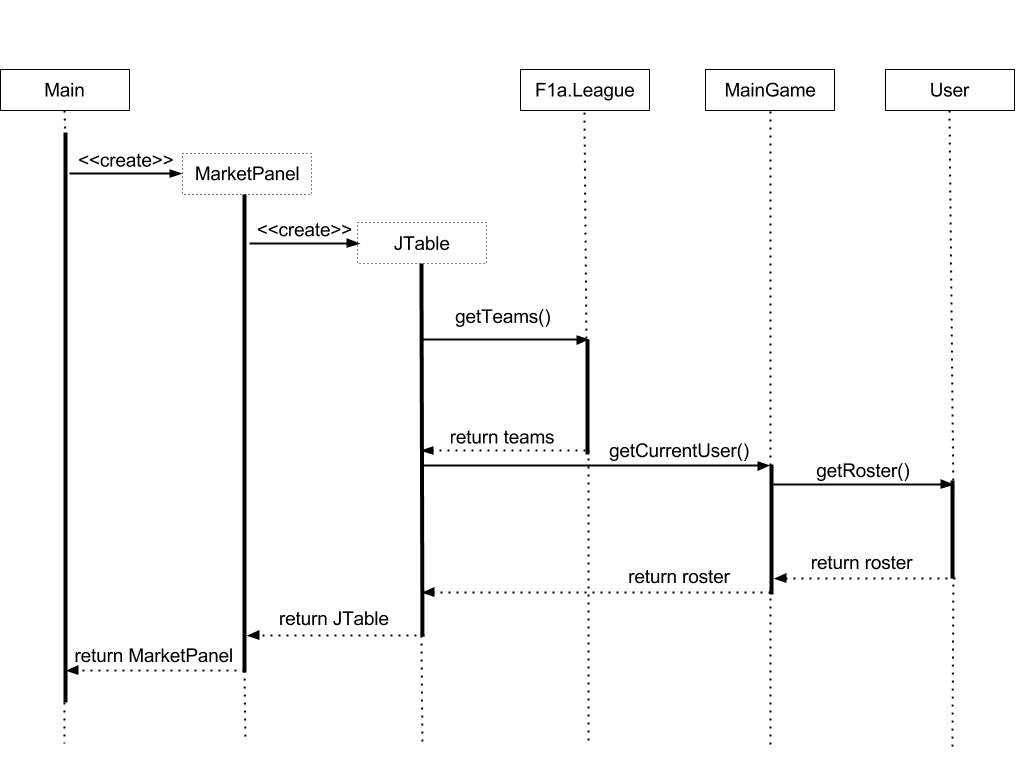
\includegraphics[width=0.75\textwidth]{img/seq_diagram_1.png}
\caption{Sequence diagram 1.}
\end{figure}
\vspace*{-1cm}
\begin{figure}[H]
\centering
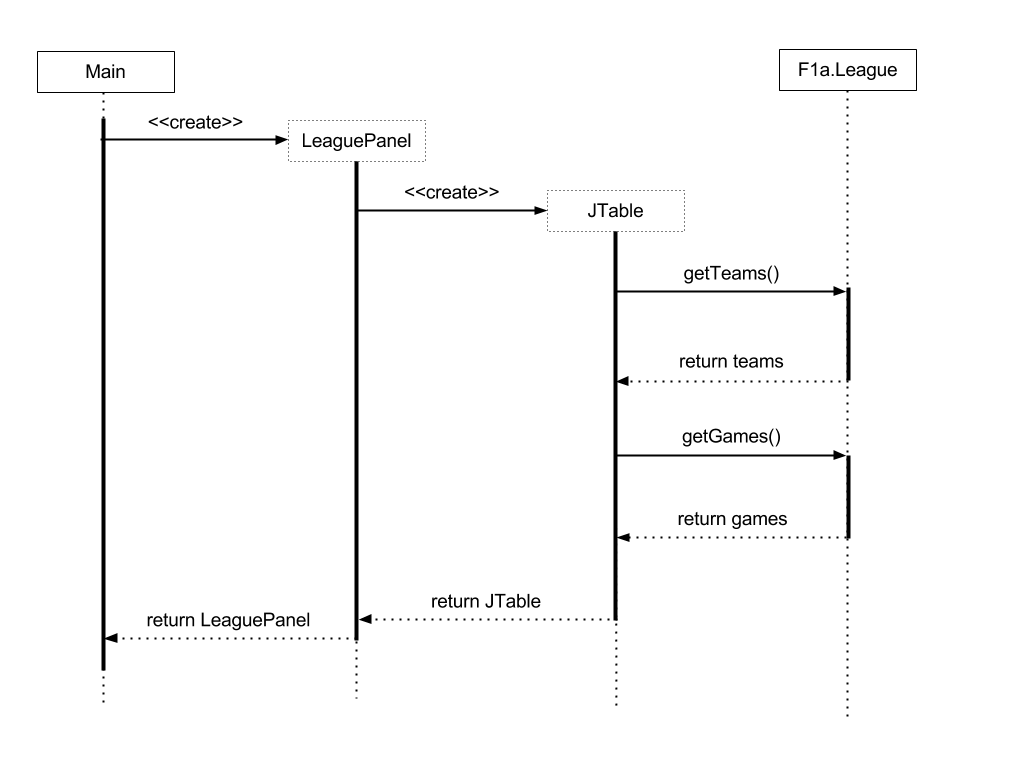
\includegraphics[width=0.75\textwidth]{img/seq_diagram_2.png}
\caption{Sequence diagram 2.}
\end{figure}

\end{document}